\documentclass[12pt,a4paper]{article}
\usepackage[T2A]{fontenc}
\usepackage[utf8]{inputenc}
\usepackage[russian]{babel}
\usepackage{amsmath}
\usepackage{amssymb}
\usepackage{graphicx}
\usepackage{floatrow}
\usepackage{booktabs}
\usepackage{wrapfig}
\usepackage{lipsum}
\usepackage{subcaption}
\usepackage{fancyhdr}
\usepackage{mathrsfs}
\usepackage{tikz}

\newcommand{\figref}[1]{(См. рис. \ref{#1})}
\newcommand{\secref}[1]{(См. раздел. \ref{#1})}

\newcommand{\e}[1]{\text{$\cdot10^{#1}$}}

\pagestyle{fancy}
\fancyhead{}
\fancyhead[L]{Работа 3.2.3}
\fancyhead[R]{}
\fancyfoot[C]{\thepage}

\author{\normalsize Выполнил: Голубович Тимур, группа Б01-108 \\
	\normalsize 26.11.2022}
\date{}

\usepackage{float}
\restylefloat{table}
\title{
	\large Отчет о выполнении лабораторной работы 3.2.3 \\
	\Large Резонанс токов в параллельном контуре \\ 
}

\begin{document}
	\maketitle
	
\section*{Цель работы}
Исследование резонанса токов в параллельном колебательном контуре с изменяемой ёмкостью, включающее получение амплитудно-частотных и фазово-частотных характеристик, а так- же определение основных параметров контура.


\section*{Оборудование и приборы}
генератор сигналов, источник тока;
нагруженный на параллельный колебательный контур с переменной ёмкостью;
двулучевой осциллограф;
цифровые вольтметры.

	
\section*{Теоретическое введение}

    В данной работе изучаются резонансные явления в параллельном колебательном контуре (резонанс токов). Синусоидальный сигнал от генератора поступает на вход управляемого напряжением источника напряжения, собранного на операционном усилителе.
    
    В колебательный контур установки добавлен постоянный резистор $R$, снижающий его
    добротность. Это сделано для упрощения процедур получения и обработки резонансных кривых. Таким образом, суммарное активное сопротивление контура принимается равным
    
    \begin{equation}
        R_{\Sigma} = R + R_L + R_S
    \end{equation}
    
    Добротность контуров тем не менее остаётся достаточно высокой, чтобы
    можно было пользоваться классическими формулами:
    
    \begin{equation}
        \mathcal{Q} = \frac{\rho}{R_{\Sigma}} = \frac{\omega_0 L}{R_{\Sigma}} 
    = \frac{1}{\omega_0 C R_{\Sigma}} \gg 1
    \end{equation}
    
    При резонансе, когда для высокодобротного контура можно положить $\omega = \omega_0$, выражения для модулей комплексных амплитуд тока и напряжения на ёмкости и их фаз принимают простой вид:
    
    \begin{equation}
        I(\omega_0) = \frac{\mathscr{E}}{R_{\Sigma}},\;\; U_C(\omega_0) = \mathcal{Q} \mathscr{E}, \;\; U_L(\omega_0) = \mathcal{Q} \mathscr{E}.
    \end{equation}

	\section*{Экспериментальная установка}

    Схема экспериментального стенда показана на рис. \ref{fig:scheme}.
    
    \begin{figure}[H]
    	\centering
    	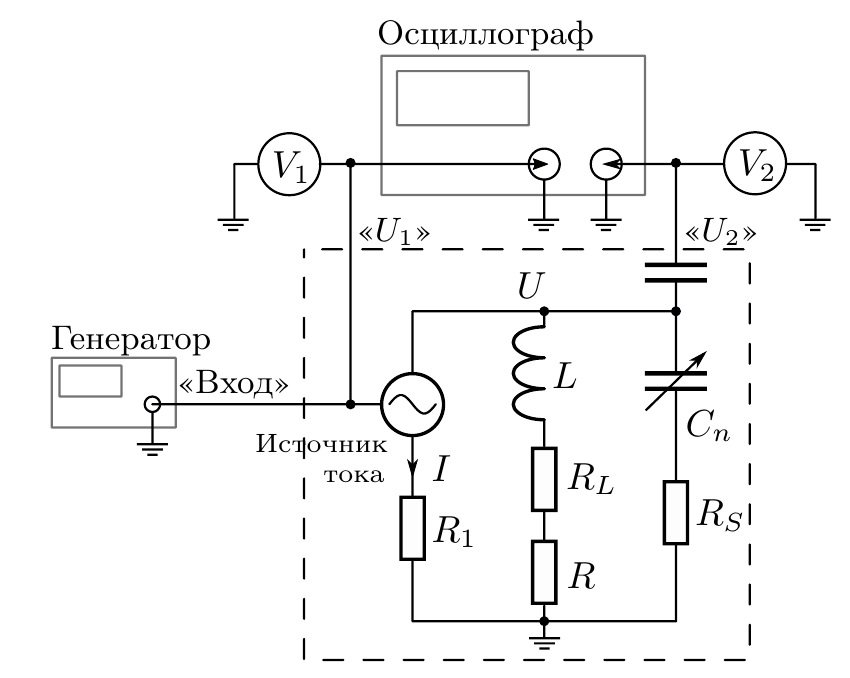
\includegraphics[scale = 0.4]{res/scheme.png}
    	\caption{Схема экспериментального стенда}
    	\label{fig:scheme}
    \end{figure}
    
   
   
   
\section*{Ход работы}

\subsection*{Измерение параметров контура}
Вначале зафиксируем сопротивления установки $R=3.5$ Ом $R_1=1008$ Ом. Для контуров с различными ёмкостями $C_n$, меняя их с помощью переключателя на блоке, измерим резонансные частоты $f_0$ и напряжения $U_C$ при установленном в напряжении $\mathscr{E}$ на выходе генератора. Для каждого значения $C_n$ по данным эксперимента проведем расчёт параметров стенда (см. таблицу \ref{tab:params}): $$L=\frac{1}{C\cdot(2\pi f)^2},$$ $$\rho=\frac{1}{C\cdot 2\pi f},$$ $$Z_{\text{рез}}=\frac{U_C}{\mathscr{E}}R_1,$$  $$\mathcal{Q}=\frac{Z_{\text{рез}}}{\rho},$$ $$R_{\Sigma}=\frac{\rho^2}{Z_{\text{рез}}},$$   $$R_{S_{\text{max}}}=\delta \cdot \rho,$$ $$R_L=R_{\Sigma}-R-R_{S_{\text{max}}}.$$

\begin{table}[H]
	\centering
	\footnotesize
	\begin{tabular}{cc}
\toprule
$r$, Ом & $R_L$, Ом \\
\midrule
12.2 & 31.5 \\
\bottomrule
\end{tabular}


	\caption{Параметры контура}
	\label{tab:params}
\end{table}



Рассчитаем средние значения $L$ и $R_L$ и их случайные погрешности для использования в дальнейшем:
$$L = 983 \pm 7 \; \text{мкГн} \;\;\; \varepsilon_L = 0.7 \%,$$
$$R_L = 2.5 \pm 0.3 \; \text{Ом} \;\;\; \varepsilon_L = 10 \%.$$

\subsection*{Измерение АЧХ}

Проведём измерения АЧХ для двух различных ёмкосей $C_2=33.2$ нФ и $C_5=67.5$ нФ. Результаты измерений занесём в таблицу \ref{tab:afc} и отобразим на графике \ref{fig:afc1}. Также вычислим резонансную частоту $f_0$ и амплитуду $U_0$ с помощью экстраполяции полиномом 4 степени (таблица \ref{tab:res}), после чего перейдём к безразмерным параметрам $\frac{f}{f_0}\left(\frac{U}{U_0}\right)$. Построим соответвующий график \ref{fig:afc2}. Определим добротность $\mathcal{Q}$ контуров по уровню $\frac{1}{\sqrt{2}}$:
    $$\mathcal{Q}_2 = 25.6 \pm 0.6 \;\;\; \varepsilon_{\mathcal{Q}_2} = 2 \%$$
    $$\mathcal{Q}_5 = 19.4 \pm 0.4 \;\;\; \varepsilon_{\mathcal{Q}_5} = 2 \%.$$

\begin{table}[H]
	\centering
	\footnotesize
	\begin{tabular}{cc|cc}
\toprule
$f$, кГц & $U_{C}$, В & $f$, кГц & $U_{C}$, В \\
\multicolumn{2}{c}{$C_2=33.2$ нФ} & \multicolumn{2}{c}{$C_5=67.5$ нФ} \\
\midrule
26.996 & 0.4713 & 18.801 & 0.2691 \\
27.183 & 0.5630 & 18.856 & 0.2842 \\
27.261 & 0.6071 & 18.883 & 0.2924 \\
27.307 & 0.6380 & 19.038 & 0.3445 \\
27.438 & 0.7250 & 19.083 & 0.3613 \\
27.536 & 0.7883 & 19.126 & 0.3781 \\
27.638 & 0.8510 & 19.196 & 0.4050 \\
27.913 & 0.9000 & 19.322 & 0.4470 \\
27.998 & 0.8660 & 19.558 & 0.4662 \\
28.086 & 0.8168 & 19.693 & 0.4336 \\
28.144 & 0.7800 & 19.737 & 0.4190 \\
28.160 & 0.7720 & 19.844 & 0.3808 \\
28.202 & 0.7460 & 19.923 & 0.3520 \\
28.325 & 0.6650 & 19.964 & 0.3340 \\
28.462 & 0.5844 & 20.141 & 0.2830 \\
28.634 & 0.5010 & 20.206 & 0.2680 \\
\bottomrule
\end{tabular}

	\caption{Измерения АЧХ}
	\label{tab:afc}
\end{table}

\begin{figure}[H]
	\centering
	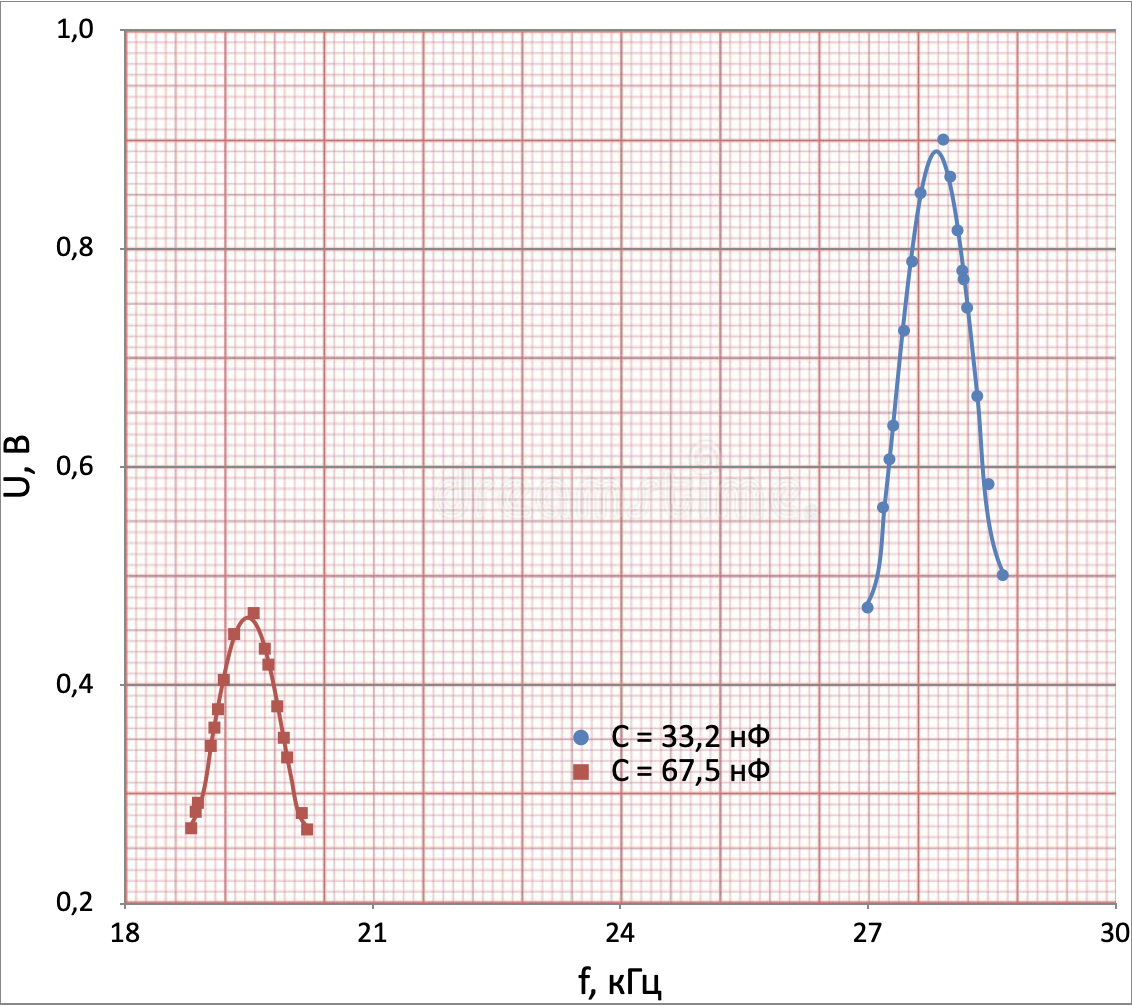
\includegraphics[width=10cm]{"src/afc1.png"}
	\caption{График АЧХ}
	\label{fig:afc1}
\end{figure}

\begin{figure}[H]
	\centering
	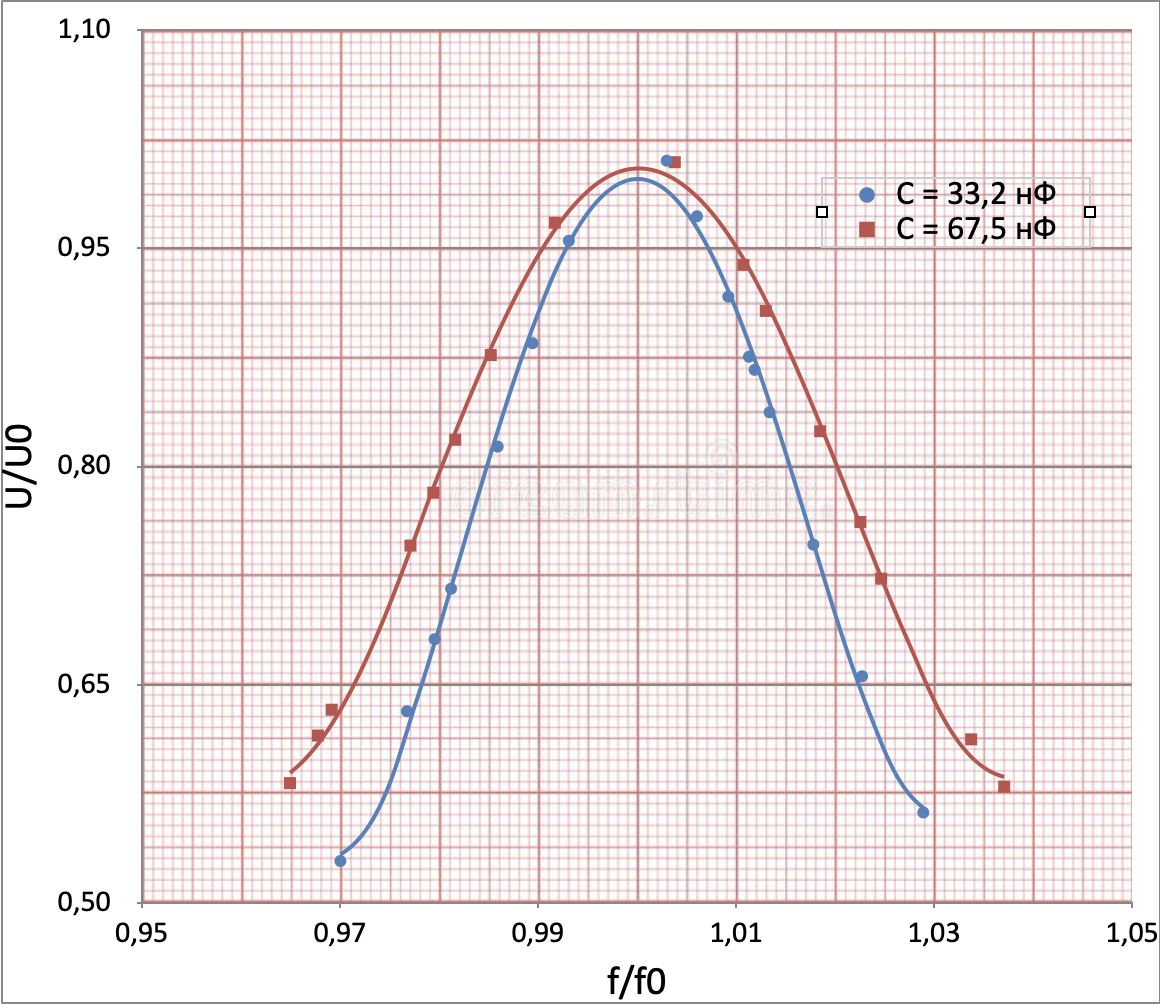
\includegraphics[width=10cm]{"src/afc2.png"}
	\caption{График АЧХ в обезразмеренных координатах}
	\label{fig:afc2}
\end{figure}

\begin{table}[H]
	\centering
	\footnotesize
	\begin{tabular}{ccc}
\toprule
 & $f_0$, кГц & $U_0$, В \\
\midrule
$C_2$  & 27.830 & 0.891 \\
$C_5$  & 19.484 & 0.462 \\
\bottomrule
\end{tabular}
	\caption{Резонансные параметры}
	\label{tab:res}
\end{table}

\subsection*{Измерение ФЧХ}

Аналогично проведём измерения для ФЧХ. Занесём их в таблицу \ref{tab:apc} и построим график ФЧХ \ref{fig:apc1} в обезразмеренных координатах $\frac{f}{f_0}\left(\frac{\Delta \phi}{\pi} \right)$. Определим добротность контура по расстоянию между точками оси $Ox$, в которых $y$ меняется от $-\frac{1}{4}$ до $\frac{1}{4}$:
    $$\mathcal{Q}_2 = 26.1 \pm 0.7 \;\;\; \varepsilon_{\mathcal{Q}_2} = 1.9 \%$$
    $$\mathcal{Q}_5 = 20.0 \pm 0.4 \;\;\; \varepsilon_{\mathcal{Q}_5} = 1.8 \%.$$

\begin{table}[H]
	\centering
	\footnotesize
	\begin{tabular}{cccc|cccc}
\toprule
$x$, дел & $x_0$, дел & $f$, кГц & $\Delta \phi$ & $x$, дел & $x_0$, дел & $f$, кГц & $\Delta \phi$ \\
\multicolumn{4}{c}{$C_2=33.2$ нФ} & \multicolumn{4}{c}{$C_5=67.5$ нФ} \\
\midrule
-10.5 & 27.2 & 18.200 & -1.213 & -8.0 & 18.9 & 26.025 & -1.330 \\
-10.0 & 26.8 & 18.474 & -1.172 & -7.7 & 18.8 & 26.350 & -1.286 \\
 -9.0 & 26.7 & 18.648 & -1.059 & -7.1 & 18.6 & 26.554 & -1.199 \\
 -8.0 & 26.3 & 18.824 & -0.955 & -6.5 & 18.3 & 26.895 & -1.116 \\
 -7.5 & 26.2 & 18.909 & -0.899 & -6.2 & 18.3 & 27.021 & -1.064 \\
 -6.3 & 26.2 & 19.057 & -0.755 & -5.0 & 18.2 & 27.285 & -0.863 \\
 -5.0 & 25.8 & 19.171 & -0.609 & -4.0 & 18.1 & 27.408 & -0.694 \\
  1.5 & 25.2 & 19.591 &  0.187 & -2.4 & 17.9 & 27.626 & -0.421 \\
  4.3 & 25.0 & 19.786 &  0.540 & -1.2 & 17.8 & 27.723 & -0.212 \\
  5.0 & 24.9 & 19.845 &  0.631 &  1.8 & 17.7 & 27.988 &  0.319 \\
  6.1 & 24.8 & 19.969 &  0.773 &  2.1 & 17.5 & 28.053 &  0.377 \\
  6.5 & 24.7 & 20.024 &  0.827 &  3.5 & 17.2 & 28.238 &  0.639 \\
  6.9 & 24.5 & 20.090 &  0.885 &  4.2 & 17.5 & 28.337 &  0.754 \\
  7.3 & 24.4 & 20.167 &  0.940 &  5.2 & 17.3 & 28.597 &  0.944 \\
  8.0 & 24.2 & 20.334 &  1.038 &  6.0 & 16.9 & 28.893 &  1.115 \\
  9.0 & 23.7 & 20.761 &  1.193 &  6.6 & 16.8 & 29.461 &  1.234 \\
\bottomrule
\end{tabular}

	\caption{Измерения ФЧХ}
	\label{tab:apc}
\end{table}

\begin{figure}[H]
	\centering
	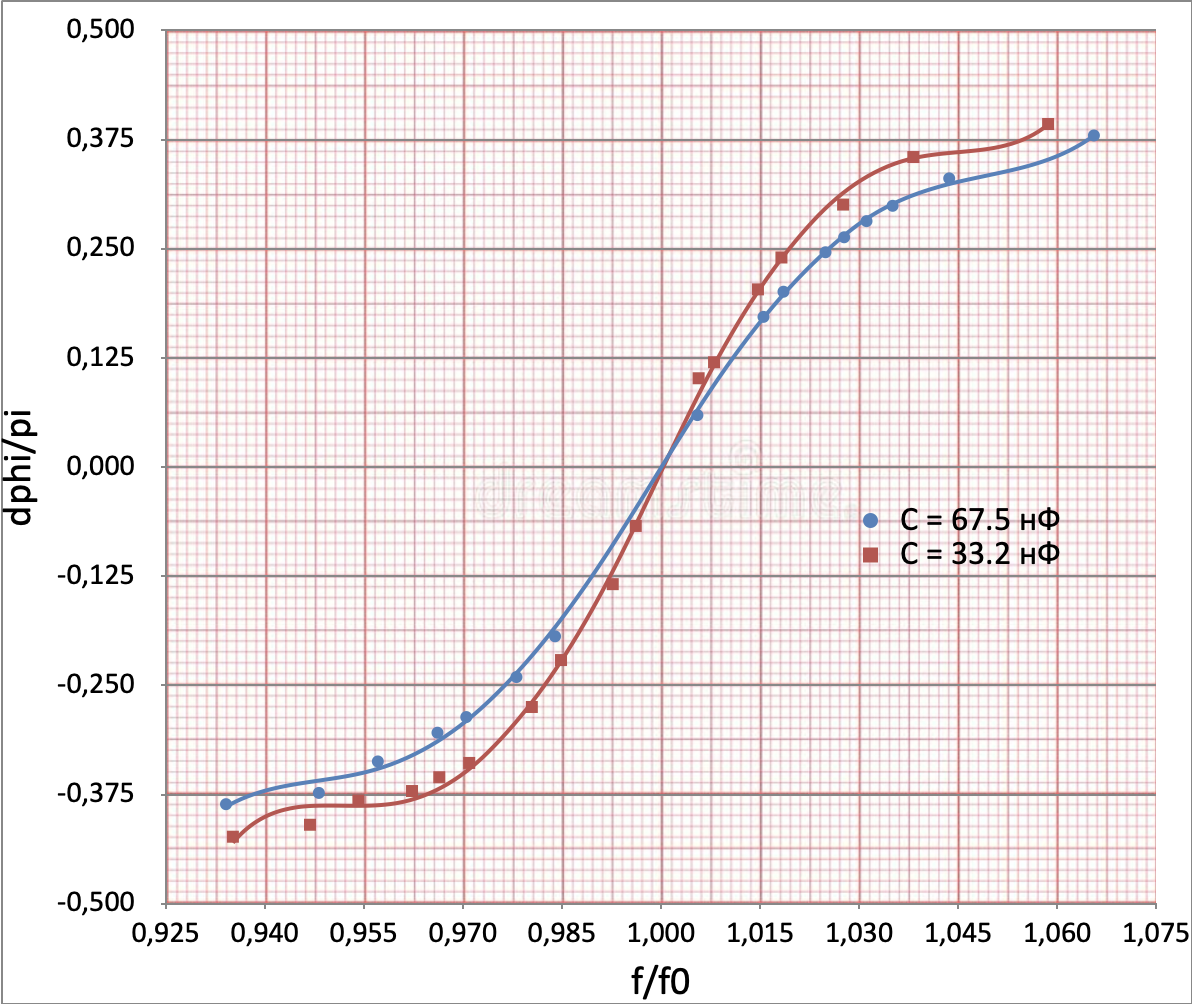
\includegraphics[width=10cm]{"src/apc1.png"}
	\caption{График ФЧХ в обезразмеренных координатах}
	\label{fig:apc1}
\end{figure}

\subsection*{Зависимость $R_L$ от $f$}

Построим график зависимости $R_L\left(f\right)$ и нанесём на него среднее значение $R_L$, вычисленное вначале. Как видно из графика \ref{fig:rl}, сопротивление катушки увеличивается с частотой.

\begin{figure}[H]
	\centering
	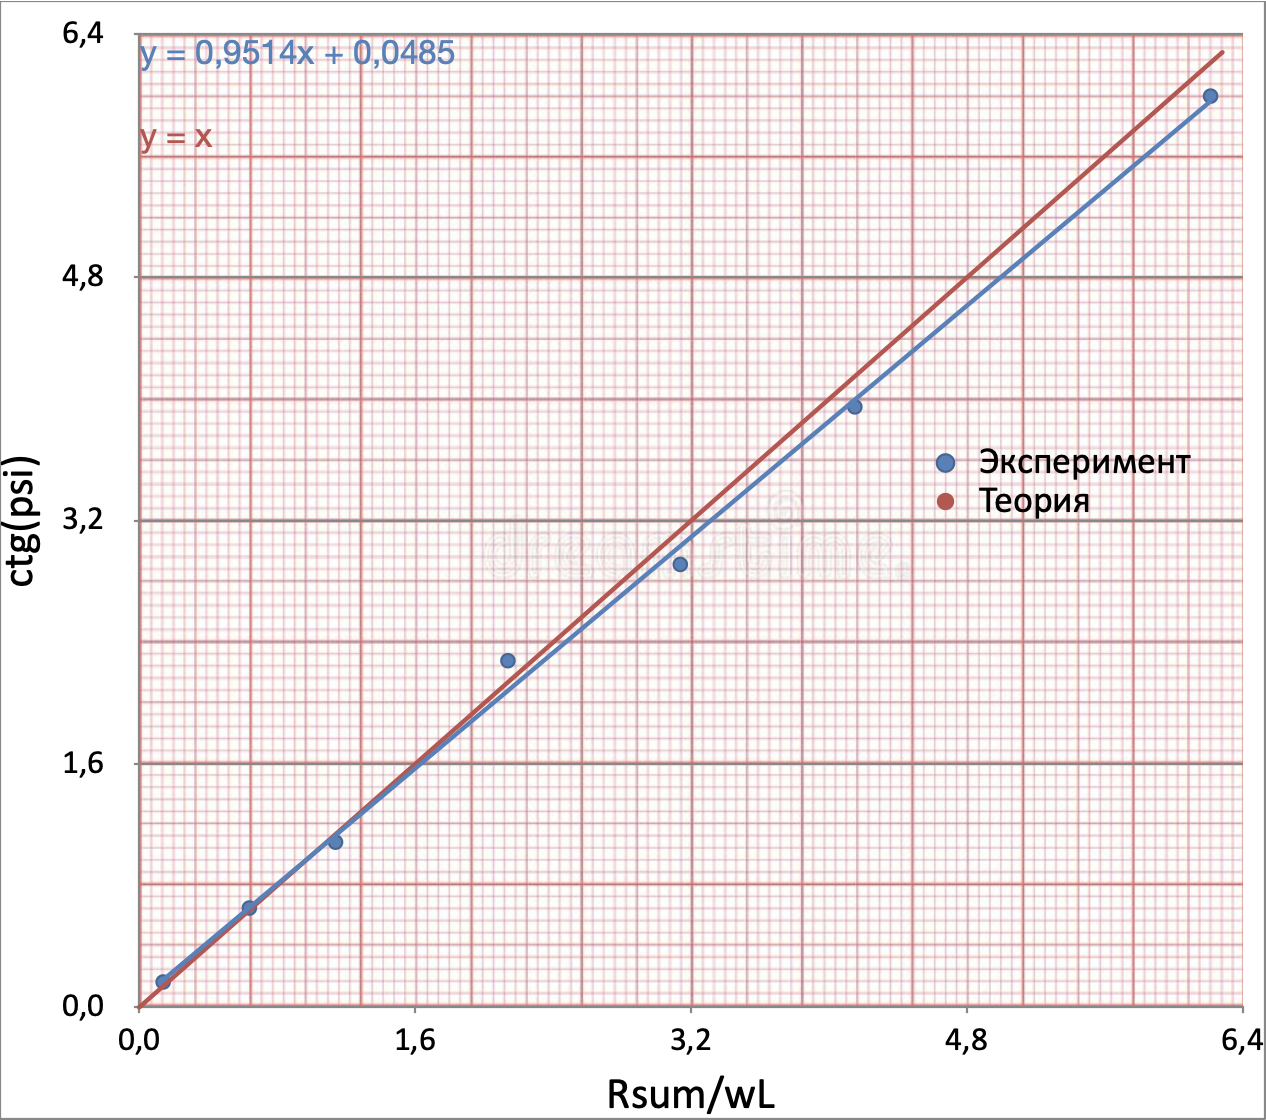
\includegraphics[width=10cm]{"src/RL.png"}
	\caption{График зависимости $R_L$ от резонансной частоты}
	\label{fig:rl}
\end{figure}

\subsection*{Векторная диаграмма}

Теперь построим векторную диаграмму для контура с наименьшей добротностью, т.е. для последнего --- $ Q_7 = 17.0 $. 

\begin{figure}[H] 
	\begin{tikzpicture} [scale = 1.8, yshift=2pt]
		\draw  (0, 0) -- (0, 2.1);
		\draw (0, 0) -- (0, - 2.1);
		\draw  (0, 0) -- (2.5, 0);
		\draw [->] (0, 0) -- (0.75, 2) node[anchor=west] {$ \vec{I_C} $};
		\draw (0, 1.3) arc (60:0: 0.6);
			\draw (0.2,1.4) node {$ \varphi_C'$};
				\draw [->] (0, 0) -- (0.06, -2) node[anchor=west] {$ \vec{I_L} $};
			\draw (0, -1.3) arc (0:30: -0.4);
			\draw (0.15,-1.4) node {$ \delta$};
			\draw [->] (0, 0) -- (0.75, 0) node[anchor=south] {$ \vec{I} $};
			\draw [->] (0, 0) -- (1.75, -0.4) node[anchor=north] {$ \vec{U} $};
				\draw (1, 0) arc (30:0: 0.6);
					\draw (1.3,-0.2) node {$ \varphi_U$};
					\end{tikzpicture}
	\caption{Векторная диаграмма}
	\label{fig:diag}
\end{figure}

Посчитаем ток $ I = \dfrac{\mathscr{E}}{R_1} = \dfrac{0.2}{1008} \approx 0.1 мА $. Его вектор равен сумме: $ \vec{I} = \vec{I_L} + \vec{I_C} $, причем сам $ \vec{I} $ расположен на оси абсцисс, а его компоненты расположены к нему под углами

\begin{equation}\label{}
\varphi_C = \dfrac{\pi}{2} - \dfrac{R + R_l}{\rho}, \quad \varphi_L = -\dfrac{\pi}{2} + \delta
\end{equation}

Здесь $ \delta \simeq 10^{-3}$ --- очень малый параметр установки, которым допустимо пренебречь при расчёте, однако можно изобразить для наглядности. Подсчитаем угол $\varphi_C' =   \dfrac{R + R_l}{\rho} \approx 0.0562 $. 

Аналогичный угол у напряжения $ \vec{U}: \varphi_U = - \dfrac{R + R_l}{\rho} $. Т.е. оно незначительно отклоняется от оси абсцисс на отрицательный угол.

Изобразим это на рисунке \ref{fig:diag}. 



\section*{Вывод}
Вначале работы были рассчитаны некоторые характерные параметры контуров для различных ёмкостей. Далее с помощью АЧХ и ФЧХ были получены значения добротностей для двух различных ёмкостей $C_2$ и $C_5$. Был построен график $R_L\left(f\right)$ и векторная диаграмма.

\newpage
\begin{thebibliography}{9}
	\bibitem{Siv} Сивухин Д. В. \emph{Общий курс физики. Том 3 Электричество и магнетизм}, 2004
	\bibitem{kirich} Кириченко Н.А. \emph{Электричество и магнетизм.}, 2011
	\bibitem{max} \emph{Лабораторный практикум по общей физике. В 3 томах. Том 2. Электричество и магнетизм: учебное пособие} под ред. А. В. Максимычева, М. Г. Никулина
\end{thebibliography}

\end{document}
